The classical advection-dispersion equation of a conservative solute in porous media can be written as \cite{jB79}

\begin{equation}\label{transport}
\frac{\partial C}{\partial t} = -\nabla\cdot(\mio{v}{}{}C)+\nabla\cdot(\mio{D}{}{} \nabla C)
\end{equation}

where $C$ is the concentration ($ML^{-3}$), $\mio{v}{}{}$ is the pore velocity vector ($ML^{-1}$), and $\mio{D}{}{}$ is the hydrodynamic dispersion tensor ($L^2T^{-1}$), t is time ($T^{2}$) and $ \nabla $is the differential operator.

%or get from section of mass transport

The random walk particle tracking (RWPT) method is issued from stochastic physics. The stochastic differential equation is \cite{Ito:51}

\begin{equation}\label{StochasticDifferentialEquation}
\mathbf{x} (t_{i}) = \mathbf{x} (t_{i-1}) + \mathbf{v} (\mathbf{x} (t_{i-1})) \Delta t + Z \sqrt {2\mathbf{D} (\mathbf{x} (t_{i-1})) \Delta t}
\end{equation}

where $\mathbf{x}$ is the coordinates of the particle location, $\Delta t$ is the time step, and $Z$ is a random number whose mean is zero and variance is unit.

It has been shown that this equation is equivalent to an equation that is slightly different from the advection-dispersion equation (\ref{transport}). To be equivalent to equation (\ref{transport}), the modified velocity \cite{wK86} and  dispersion tensor \cite{jB79} are expressed as

\begin{equation}\label{ModifiedVelocity}
\mathbf{v}_i^* = \mathbf{v}_i + \sum_{j=1}^{3}\frac{\partial \mathbf{D} _{ij}}{\partial x _j}
\end{equation}

\begin{equation}\label{DispersionTensor}
\mathbf{D} _{ij} = \alpha _T |\mio{v}{}{}|\delta _{ij} + (\alpha _L - \alpha _T)\frac {\mathbf{v}_i \mathbf{v}_j}{|\mio{v}{}{}|} + \mathbf{D}^d _{ii}
\end{equation}

where $\delta _{ij}$ is the Kronecker symbol, $\alpha _L$ is the longitudinal dispersivity, $\alpha _T$ is the transverse dispersivity, $D^d _{ij}$ is the tensor of molecular diffusion coefficient, and $\mathbf{v}_i$ is the component of the mean pore velocity in the $i$th direction.

The equivalent stochastic differential equation to (\ref{transport}) in three dimensional problems can be written as \cite{aT90,eL96,wK88}

\begin{equation}\label{ModifiedStochasticDifferentialEquation}
\begin{array}{llllll}
x _{t+\Delta t} & =x _{t}+ \left(\mathbf{v}_x(x _t,y _t,z _t,t) + \frac{\partial D _{xx}}{\partial x} + \frac{\partial D _{xy}}{\partial y} + \frac{\partial D _{xz}}{\partial z} \right ) \Delta t \\
&\quad + \sqrt{2D _{xx} \Delta t }Z _1 + \sqrt{2D _{xy} \Delta t }Z _2 + \sqrt{2D _{xz} \Delta t }Z _3 \\
y _{t+\Delta t} & =y _{t}+ \left(\mathbf{v}_y(x _t,y _t,z _t,t) + \frac{\partial D _{yx}}{\partial x} + \frac{\partial D _{yy}}{\partial y} + \frac{\partial D _{yz}}{\partial z} \right ) \Delta t \\
&\quad + \sqrt{2D _{yx} \Delta t }Z _1 + \sqrt{2D _{yy} \Delta t }Z _2 + \sqrt{2D _{yz} \Delta t }Z _3 \\
z _{t+\Delta t} & =z _{t}+ \left(\mathbf{v}_z(x _t,y _t,z _t,t) + \frac{\partial D _{zx}}{\partial x} + \frac{\partial D _{zy}}{\partial y} + \frac{\partial D _{zz}}{\partial z} \right ) \Delta t \\
&\quad + \sqrt{2D _{zx} \Delta t }Z _1 + \sqrt{2D _{zy} \Delta t }Z _2 + \sqrt{2D _{zz} \Delta t }Z _3 \\
\end{array}
\end{equation}

where $Z_{i}$ is a random number whose mean is zero and variance is unit.

Together with equation (\ref{DispersionTensor}), the spatial derivatives of the dispersion coefficients can be expressed as a function of the derivatives of velocity. Note that to obtain the derivatives of velocity, velocity has to be continuous mathematically. For this end, we interpolate velocity at any location in an element from the known velocity at the element nodes.

%\ref{fluid momentum}

Since the proposed RWPT method makes use of the FEM for velocity estimation, the derivative of velocity within each element is computed as in Fig.~\ref{DerivativeVelocity} and written as

\begin{equation}\label{DerivativeVelocityNotZero}
\begin{array}{ll}
\frac {\partial \mathbf{v}_x}{\partial x} = & \frac {\mathbf{v}(x_R) - \mathbf{v}(x_L)}{l _x}; \quad
\frac {\partial \mathbf{v}_y}{\partial y} = \frac {\mathbf{v}(y _U) - \mathbf{v}(y _D)}{l _y}; \quad
\frac {\partial \mathbf{v}_z}{\partial z} = \frac {\mathbf{v}(z _N) - \mathbf{v}(z _S)}{l _z} \\
& \frac {\partial \mathbf{v}_x}{\partial y} = \frac {\partial \mathbf{v}_x}{\partial z} =
\frac {\partial \mathbf{v}_y}{\partial z} = \frac {\partial \mathbf{v}_y}{\partial x} =
\frac {\partial \mathbf{v}_z}{\partial x} = \frac {\partial \mathbf{v}_z}{\partial y}
\simeq 0
\end{array}
\end{equation}

where $x _L$ and $x _R$ are the intersectional points of the element edges with an extension of a  line parallel to the global $x$ axis at which velocities are $\mathbf{v}(x _L)$ and $\mathbf{v}(x _R)$, $y _D$ and $y _U$ are the intersectional points of the element edge from down to up with extension of the line parallel to the global $y$ axis at which velocities are $\mathbf{v}(y _D)$ and $\mathbf{v}(y _U)$, $z _S$ and $z _N$ are the intersectional points of the element edge from south to north with extension of the line parallel to the global $z$ axis at which velocities are $\mathbf{v}(z _S)$ and $\mathbf{v}(z _N)$, and $l _x$, $l _y$, and $l _z$ are the length of each intersectional line respectively.

\begin{figure}[htbp!]
\centering
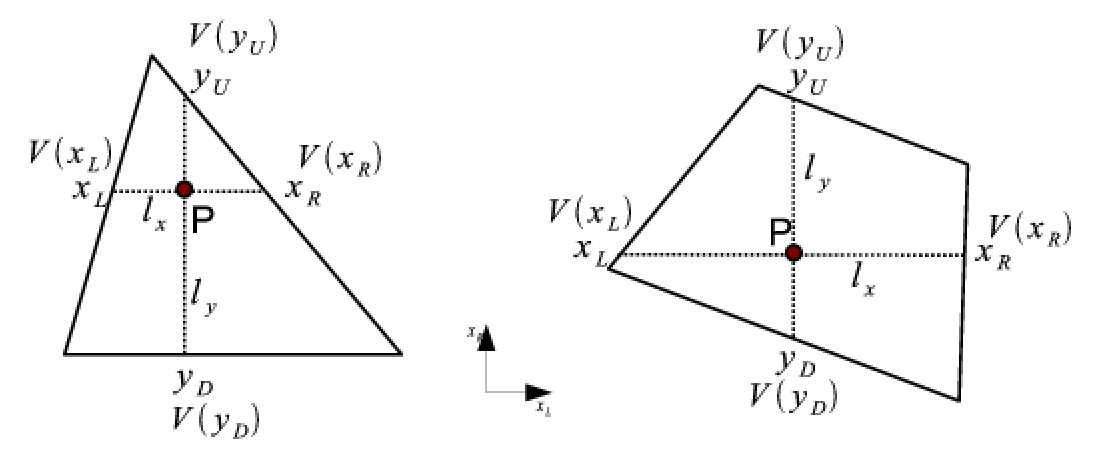
\includegraphics[scale=0.60]{PART_II/C/DerivativeScheme.eps}
\caption{Spatial derivatives of velocity for a particle in triangular and quadrilateral elements ( V is velocity)}
\label{DerivativeVelocity}
\end{figure}

Thus, the derivatives of the dispersion coefficients are as follows \cite{hH02}

\begin{equation}\label{DerivativeDispersionCoefficient}
\begin{array}{lllllllll}
& \frac{\partial D _{xx}}{\partial x}=\mathbf{v}_x\frac{\partial \mathbf{v}_x}{\partial x}\left [
\alpha _L \left (\frac {2}{\mathbf{v}} - \frac {\mathbf{v}_x ^2}{\mathbf{v}^3} \right ) - \alpha _T \frac {\mathbf{v}_y ^2 + \mathbf{v}_z ^2}{\mathbf{v}^3} \right ] \\
& \frac{\partial D _{xy}}{\partial y}=(\alpha _L - \alpha _T)\left [\frac{\partial \mathbf{v}_y}{\partial y}
\frac{\mathbf{v}_x}{\mathbf{v}} - \frac{\mathbf{v}_x \mathbf{v}_y^2}{\mathbf{v}^3} \frac{\partial \mathbf{v}_y}{\partial y} \right ] \\
& \frac{\partial D _{xz}}{\partial z}=(\alpha _L - \alpha _T)\left [\frac{\partial \mathbf{v}_z}{\partial z}
\frac{\mathbf{v}_x}{\mathbf{v}} - \frac{\mathbf{v}_x \mathbf{v}_z^2}{\mathbf{v}^3} \frac{\partial \mathbf{v}_z}{\partial z} \right ] \\
& \frac{\partial D _{yy}}{\partial y}=\mathbf{v}_y\frac{\partial \mathbf{v}_y}{\partial y}\left [
\alpha _L \left (\frac {2}{\mathbf{v}} - \frac {\mathbf{v}_y ^2}{\mathbf{v}^3} \right ) - \alpha _T \frac {\mathbf{v}_x ^2 + \mathbf{v}_z ^2}{\mathbf{v}^3} \right ] \\
& \frac{\partial D _{yx}}{\partial x}=(\alpha _L - \alpha _T)\left [\frac{\partial \mathbf{v}_x}{\partial x}
\frac{\mathbf{v}_y}{\mathbf{v}} - \frac{\mathbf{v}_y \mathbf{v}_x^2}{\mathbf{v}^3} \frac{\partial \mathbf{v}_x}{\partial x} \right ] \\
& \frac{\partial D _{yz}}{\partial z}=(\alpha _L - \alpha _T)\left [\frac{\partial \mathbf{v}_z}{\partial z}
\frac{\mathbf{v}_y}{\mathbf{v}} - \frac{\mathbf{v}_y \mathbf{v}_z^2}{\mathbf{v}^3} \frac{\partial \mathbf{v}_z}{\partial z} \right ] \\
& \frac{\partial D _{zz}}{\partial z}=\mathbf{v}_z\frac{\partial \mathbf{v}_z}{\partial z}\left [
\alpha _L \left (\frac {2}{\mathbf{v}} - \frac {\mathbf{v}_z ^2}{\mathbf{v}^3} \right ) - \alpha _T \frac {\mathbf{v}_x ^2 + \mathbf{v}_y ^2}{\mathbf{v}^3} \right ] \\
& \frac{\partial D _{zx}}{\partial x}=(\alpha _L - \alpha _T)\left [\frac{\partial \mathbf{v}_x}{\partial x}
\frac{\mathbf{v}_z}{\mathbf{v}} - \frac{\mathbf{v}_z \mathbf{v}_x^2}{\mathbf{v}^3} \frac{\partial \mathbf{v}_x}{\partial x} \right ] \\
& \frac{\partial D _{zy}}{\partial y}=(\alpha _L - \alpha _T)\left [\frac{\partial \mathbf{v}_y}{\partial y}
\frac{\mathbf{v}_z}{\mathbf{v}} - \frac{\mathbf{v}_z \mathbf{v}_y^2}{\mathbf{v}^3} \frac{\partial \mathbf{v}_y}{\partial y} \right ] \\
\end{array}
\end{equation}

Because velocity is not derivable at the interface of two adjacent element in a nonuniform flow, computing dispersion coefficient derivatives by using a finite element approach would yield erroneous values \cite{hH02}. To prevent the errors, a particle is coded to have information of an element index and the velocity estimation is continuous even at the elemental boundaries in this method. Thus, the derivatives of dispersion coefficients will be computed accordingly. This is an improved approach from the work by \cite{hH02}.
